\chapter{Simulation and Evaluation of Renewable Energy Communities: CityLearn v3}
\label{chap:simulator}
\markboth{Simulation and Evaluation Environment}{Simulation and Evaluation Environment}

% Keep displayed equations with the opening of their symbol definitions.
\begingroup
\raggedbottom
\postdisplaypenalty=10000

The architecture in Chapter~\ref{chap:energAIze} places simulation between the preparation of \gls{rec} data and the evaluation of a controller. This chapter develops that experimental environment: the extensions to CityLearn, the \gls{rec} datasets, and the methods used to check the simulator and compare control decisions. Together, these provide the experimental foundation for the learning methods in Chapters~\ref{chap:control-benchmark} and~\ref{chap:ti-marl}.

\section{Development of the Simulation Environment}
\label{sec:sim-research-contribution}
\label{sec:sim-motivation}
\label{sec:sim-inherited-gap}
\label{sec:sim-lineage}
\label{sec:sim-sota}
\label{sec:sim-iterative-instrument}

Preparing a controller for operation requires an environment in which its decisions have consequences over time. Charging a vehicle now changes the energy still needed before departure; using a battery changes the flexibility available later; and sharing \gls{pv} production changes the exchanges of several members. In the development process described in Chapter~\ref{chap:energAIze}, simulation provides this continuity. It allows a controller to learn from repeated interactions and to be evaluated under specified \gls{rec} conditions before it is selected for deployment.

An established building-energy environment, CityLearn, provided the starting point. Its building and storage models, common controller interface, and energy indicators already supported multi-building control studies \parencite{vazquezcanteli2019citylearn,nweye2025citylearnv2}. Shared tasks and datasets, including the CityLearn Challenge, had also established a common setting for comparing research methods \parencite{nagy2021citylearnchallenge}. Developing within this environment connected the work to an existing research community and allowed the new capabilities to be used alongside established models and controllers.

The contribution developed in this thesis extends that foundation with \gls{rec} resources, operating events, controller interfaces, and evaluation methods. It began with the integration of \glspl{ev} through EVLearn, which introduced chargers, connection schedules, departure requirements, and bidirectional charging \parencite{fonseca2025evlearn}. Work on \gls{rec} control, informed by \gls{opeva} and DemFlex, then required a broader representation of how installations operate. Members could join or leave, equipment could change, flexible appliances had complete programmes to deliver, and local sharing affected individual costs. Measurements and commands could also fail. These conditions shaped the subsequent development of CityLearn v3 and the experiments it needed to support \parencite{fonseca2026citylearnv3}.

Accommodating them involved changes across the simulation process. Installing a charger, for example, introduces a physical resource, an action that a controller can request, and future charging services whose outcomes must be recorded. Its identity and activation time therefore have to agree across scenario loading, state progression, controller inputs, and evaluation. Similar connections arise when a member leaves or an action cannot be applied. The work extended these parts together so that an experiment could follow a change from its declaration to its effect on energy use and participant service.

These extensions give the \glspl{rq} in Chapter~\ref{chap:introduction} concrete experimental settings. A changing resource collection exposes the adaptation and computational demands of scalability; electrical limits and participant services establish the conditions for examining safety; and repeatable failures make robustness comparisons possible. The controller interface also carries the resource and action descriptions needed by the deployment process in Chapter~\ref{chap:energAIze}. The following control chapters use this foundation to investigate how the methods respond.

\label{sec:sim-public-release}
The resulting software was first distributed by the \gls{softcps} Research Group as the \gls{softcps} \gls{rec} Simulator \parencite{softcps2026simulatorrepo,softcps2026pypi}. In September 2026, this development line was incorporated into the official CityLearn version~3, distributed as \texttt{citylearn} \parencite{citylearn2026v3release}. Its Gymnasium interface, examples, documentation, and tests make the extensions available through the established project \parencite{citylearn2026official}. The contribution thus provides both the experimental environment used in this thesis and reusable modelling and evaluation capabilities for other \gls{rec}-control studies.

\section{Community Modelling and Simulator Architecture}
\label{sec:sim-architecture}
\label{sec:sim-deployment-pipeline}

The simulator represents buildings and their resources within one or more \glspl{rec}. In the scenarios used here, each member is represented by one building site, with a local agent managing that site's assets. This modelling convention instantiates the distinctions in Section~\ref{sec:ch2-rec-members}; it does not equate members, sites, and agents in the general definition. A scenario supplies their data, connections, services, and operating events; a controller receives observations and proposes actions as the simulation advances. Figure~\ref{fig:sim-architecture} locates these interactions. Each \gls{rec} retains its own members, local sharing, and outcomes, while a common environment can advance several \glspl{rec} together.

The changes shown in the figure are part of the model: a member leaves, a charger is installed, and data or equipment become unavailable. Each changes a different aspect of the decision faced by the controller. The following subsections explain how these conditions are represented and how the implementation makes their consequences available for subsequent experiments.

\begin{figure}[htbp]
\centering
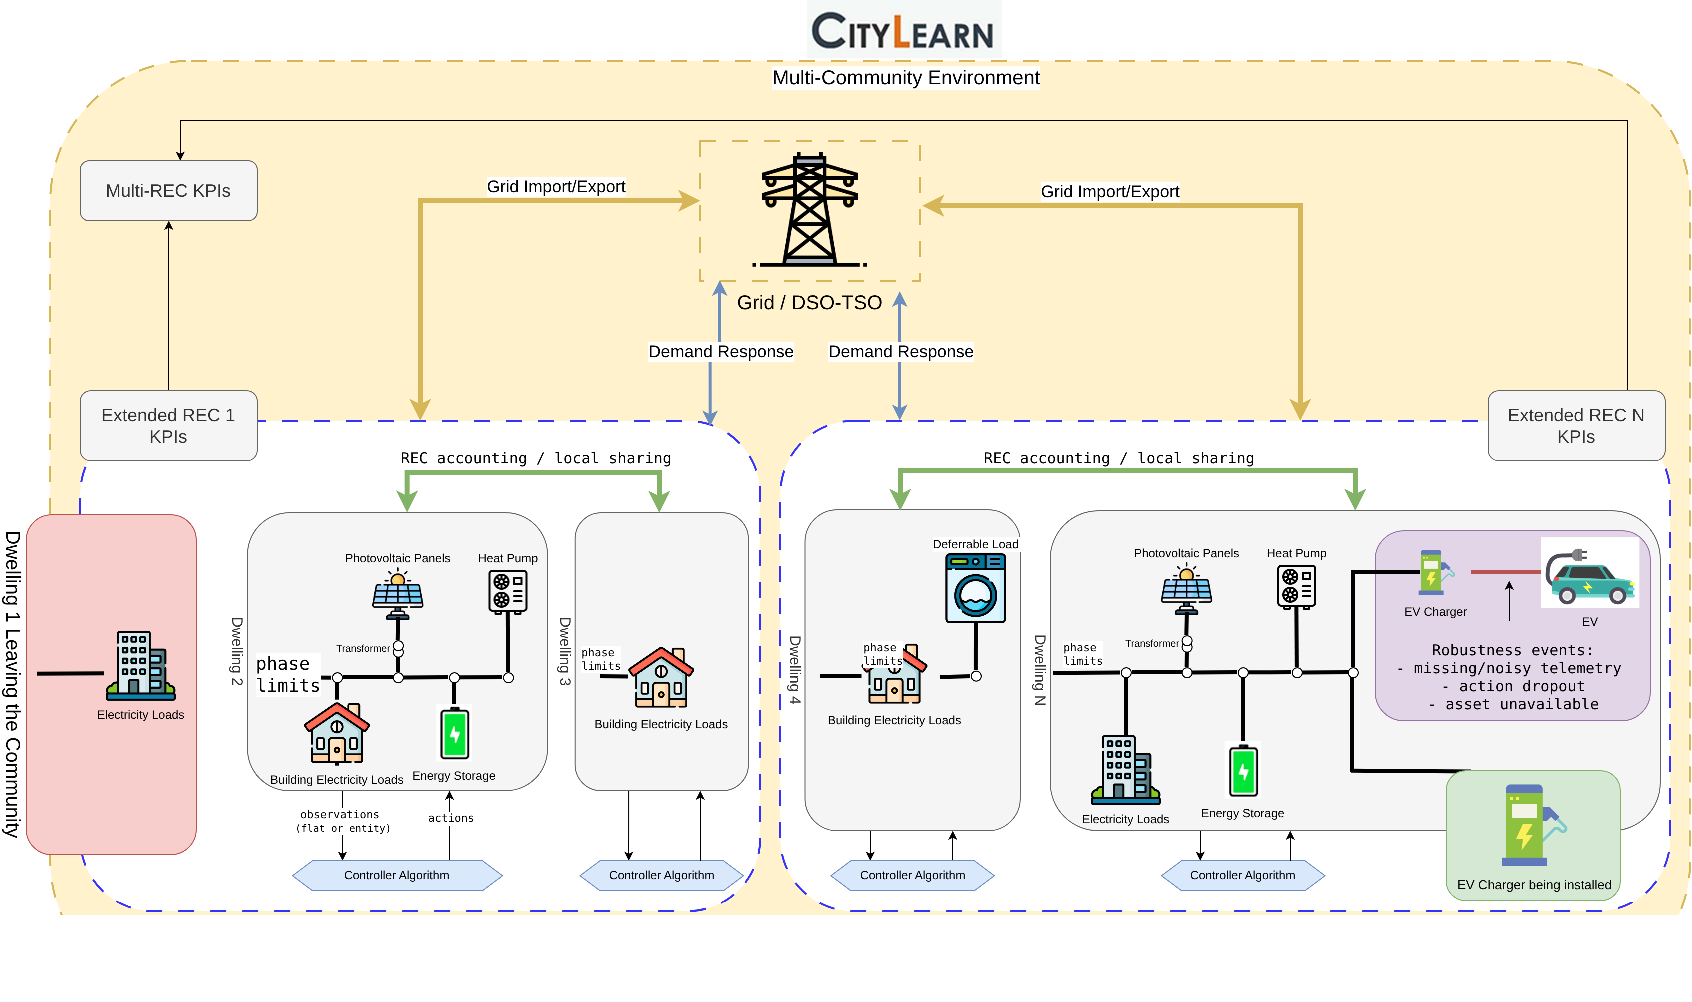
\includegraphics[width=1.0\textwidth]{simulator-environment-architecture.pdf}
\caption{Representation of one or more \glspl{rec} in CityLearn v3. Reproduced from \textcite{fonseca2026citylearnv3}.}
\label{fig:sim-architecture}
\end{figure}

\subsection{Scenarios, Time, and the Simulation Step}
\label{sec:sim-contracts}

A scenario combines time series with the information needed to interpret them. It identifies the buildings and equipment, their capacities and connections, the services to deliver, the observations exposed to a controller, and the events active during the episode. This configuration distinguishes two experiments that use identical household demand but differ in charging availability, an electrical limit, or a missing measurement.

\begin{samepage}
At timestep $t$, the simulator first resolves scheduled changes and constructs the available observations. The controller then proposes an action, which passes through the applicable feasibility and availability rules before the resources advance:
\begin{equation}
\begin{aligned}
\tilde{o}_t&=\mathcal{O}(x_t,w_t,e_t), & a_t^{\mathrm{req}}&=\pi(\tilde{o}_t),\\
a_t^{\mathrm{app}}&=\Gamma(a_t^{\mathrm{req}},x_t,e_t), & (x_{t+1},y_t)&=F(x_t,a_t^{\mathrm{app}},w_t,e_t).
\end{aligned}
\label{eq:sim-step-contract}
\end{equation}
Here, $x_t$ is the represented physical and service state, $w_t$ contains external inputs such as demand and weather, and $e_t$ contains active events. The observation function $\mathcal{O}$ produces the controller-visible information $\tilde{o}_t$, and policy $\pi$ returns requested action $a_t^{\mathrm{req}}$. Operator $\Gamma$ accounts for the configured limits, availability, and command handling to obtain applied action $a_t^{\mathrm{app}}$. The transition function $F$ produces the next state $x_{t+1}$ and the physical, service, and accounting outcomes $y_t$.\par
\end{samepage}

For the charging example, the \gls{soc} after an interval depends on the power actually applied. Retaining the original request makes it possible to distinguish a controller that respects the connection limit from one whose proposals repeatedly require correction, even when both produce the same physical trajectory. This separation gives the safety experiments access to the decision and its execution. It corresponds to the controller, supervisor, and equipment roles described in Section~\ref{sec:energaize-runtime}.

Time and units are part of this interpretation. Power and instantaneous limits use kW, interval energy uses kWh, prices use currency/kWh, and carbon intensity uses kgCO$_2$/kWh. Average power converts to interval energy through
\begin{samepage}
\begin{equation}
E_t=P_t\frac{\Delta t}{3600},
\label{eq:sim-power-energy}
\end{equation}
where $E_t$ is energy in kWh during interval $t$, $P_t$ is its average power in kW, and $\Delta t$ is the interval duration in seconds. The factor 3600 converts seconds to hours. A \SI{7.2}{\kilo\watt} charger consequently supplies \SI{1.8}{\kilo\watt\hour} in 15 minutes or \SI{0.03}{\kilo\watt\hour} in 15 seconds.\par
\end{samepage}

The same care applies to \gls{pv} inputs. A normalised production profile is scaled by installed capacity, whereas an absolute production series already describes the site's output. The loader checks the declared clock, timestamp spacing, and episode bounds. Columnar storage and windowed loading make short timesteps practical for repeated learning experiments without requiring each run to process an entire high-frequency dataset.

Figure~\ref{fig:sim-high-frequency} illustrates why temporal resolution matters to safety-sensitive studies. It represents the same synthetic annual trace at one-hour, 15-minute, and 15-second resolution. The annual energy is preserved, while the visible peak rises from 96.8 to 188.2 and 281.5~kW as shorter intervals retain events hidden by averaging. A simulator intended to study electrical headroom therefore needs an explicit clock and consistent energy accounting; the experiment can then choose the resolution appropriate to its control question \parencite{fonseca2026citylearnv3}.

\begin{figure}[htbp]
\centering
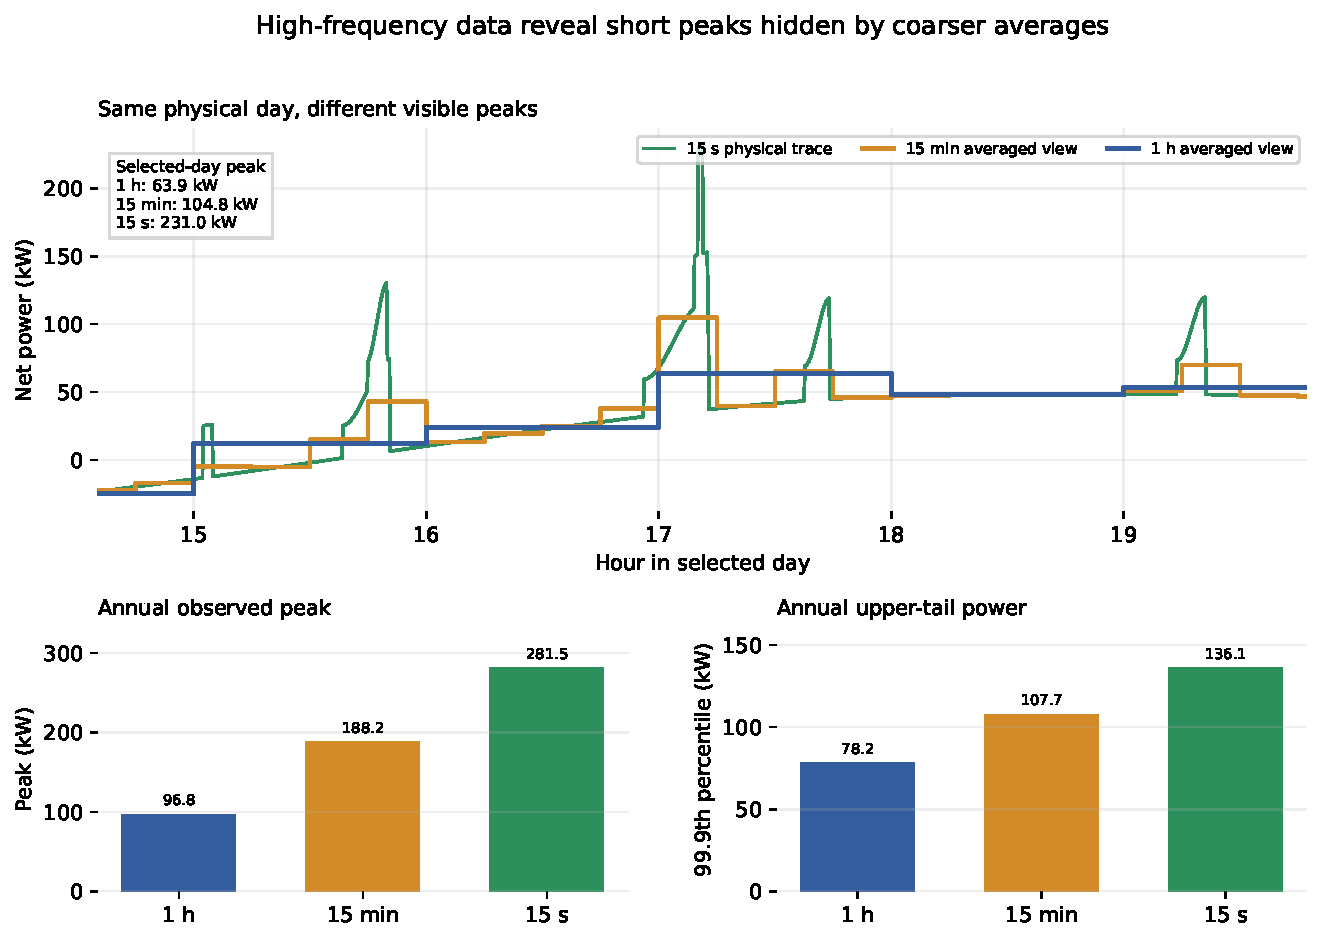
\includegraphics[width=0.96\textwidth]{simulator-high-frequency.pdf}
\caption{Peak visibility at three temporal resolutions of the same synthetic annual trace.}
\label{fig:sim-high-frequency}
\end{figure}

\subsection{Resources, Electrical Limits, and Participant Services}

Buildings retain background demand, \gls{pv} generation, grid exchange, and their available flexibility resources. Inherited thermal and storage components preserve compatibility with established CityLearn studies. The extensions developed here connect stationary storage, \gls{ev} charging, and complete appliance cycles to the services and electrical conditions of each installation.

\paragraph{Stationary storage and electrical headroom.}
A stationary battery has an energy capacity, charging and discharging power, efficiency, and state-of-charge limits. Its admissible exchange changes with stored energy and with the headroom available at the building. Charging a battery and a vehicle at the same time may therefore require less power than either device could accept alone.

\begin{samepage}
The electrical model represents total import/export limits and, where configured, separate limits for each phase. With import taken as positive, the limits are
\begin{equation}
-X_b^{\max}\leq P_{b,t}\leq I_b^{\max},\qquad
-X_{b,\phi}^{\max}\leq P_{b,\phi,t}\leq I_{b,\phi}^{\max}\quad\forall\phi\in\Phi_b.
\label{eq:sim-electrical-limits}
\end{equation}
Here, $b$ is a building, $t$ the timestep, and $\Phi_b$ its electrical phases. Total and phase power are $P_{b,t}$ and $P_{b,\phi,t}$; $I^{\max}$ and $X^{\max}$ denote the positive import and export limits. All powers are in kW.\par
\end{samepage}

If the house already imports \SI{4}{\kilo\watt} on a phase limited to \SI{7}{\kilo\watt}, a \SI{7.2}{\kilo\watt} charging request has only \SI{3}{\kilo\watt} of headroom. Representing the connection as well as the device rating exposes this competition between simultaneous uses. Requested pressure measures the excess before constraint handling, while residual violation measures exceedance in the applied trajectory, including cases where background demand alone exceeds a limit. Section~\ref{sec:sim-service-evaluation} defines how these quantities enter the safety comparison.

\paragraph{Vehicles and charging sessions.}
A charging session specifies the connected vehicle, arrival \gls{soc}, departure time, requested departure state, and applicable power bounds. These quantities determine the remaining energy requirement and the time in which it can be met. As 08:00 approaches, the same postponement that was harmless at 18:00 may make the target unreachable. The simulator follows battery response through the session and evaluates service at departure.

The model gives the vehicle, physical charging port, and session separate identities. When the example vehicle leaves at 08:00, another vehicle may use the same port later that day: the service requirement changes while the installed equipment remains the same. Adding a second port changes the resources the controller can address. This separation allows experiments to vary service demand and resource composition independently, and to associate each departure outcome with the correct request.

The vehicle catalogue can link visits across sites. In the dataset runtime used here, each session supplies its arrival \gls{soc}; battery evolution then follows the applied charging power until departure. A window beginning during an occupied session uses the corresponding boundary state. The departure record compares achieved \gls{soc} with the requirement and gives the remaining energy deficit. Lower electricity consumption can therefore be read alongside the service actually delivered.

\paragraph{Deferrable appliances.}
A deferrable appliance offers a different decision: when to begin a complete programme. A cycle catalogue supplies the interval-energy profile and duration, while a request supplies an admissible start window, completion deadline, and service priority. Choosing a start commits the simulation to that programme. This preserves its energy and duration when a controller shifts it towards a favourable price or a period of solar production.
\begin{samepage}
\begin{equation}
t_c^{\mathrm{earliest}}\leq s_c\leq t_c^{\mathrm{latest}},\qquad s_c+d_c-1\leq t_c^{\mathrm{deadline}}.
\label{eq:sim-deferrable-feasibility}
\end{equation}
Here, $c$ identifies a requested cycle, $s_c$ is its selected start timestep, and $d_c$ is its duration in timesteps. The quantities $t_c^{\mathrm{earliest}}$, $t_c^{\mathrm{latest}}$, and $t_c^{\mathrm{deadline}}$ are the earliest start, latest start, and final admissible completion timestep. For a discrete profile $q_{c,\tau}$, the index $\tau$ denotes the interval within the cycle and $q_{c,\tau}$ gives its energy demand.\par
\end{samepage}

\begin{figure}[htbp]
\centering
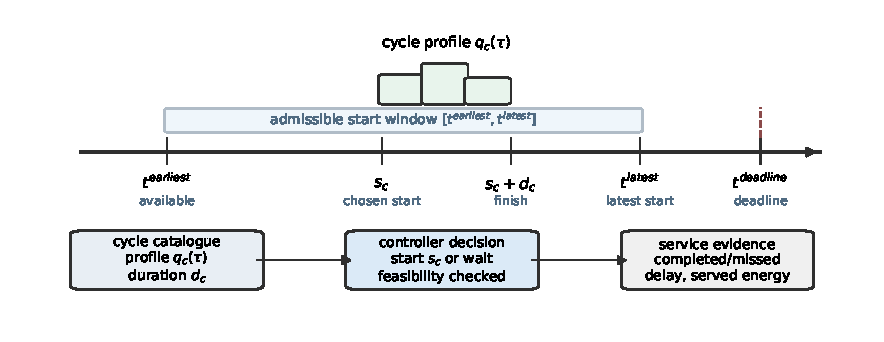
\includegraphics[width=0.96\textwidth]{simulator-deferrable-cycle.pdf}
\caption{A complete appliance programme scheduled within its admissible start window.}
\label{fig:sim-deferrable-cycle}
\end{figure}

Figure~\ref{fig:sim-deferrable-cycle} relates the scheduling choice to the complete service. Once a cycle starts, its progress is followed alongside electrical limits. Completed and missed cycles, delay, delivered energy, and unserved energy make the consequence visible. This permits the evaluation to distinguish demand shifted successfully from demand simply left unserved.

\subsection{Local Sharing and Demand-Response Services}

An aggregate \gls{rec} balance can hide simultaneous import and export by different participants. The simulator calculates local sharing in each interval, preserving the coincidence of demand and surplus, and settles that exchange at member level. A neighbour can then benefit from solar production when it is available, while storage and scheduling determine how much demand can be moved into that interval. Member demand, local exchange, and residual grid exchange remain separate quantities.

\begin{samepage}
For the active member set $\mathcal{C}_t$, local sharing is bounded by simultaneous demand and surplus:
\begin{equation}
\begin{aligned}
D_{\mathcal{C},t}&=\sum_{b\in\mathcal{C}_t}\max(E^{\mathrm{net}}_{b,t},0),\\
S_{\mathcal{C},t}&=\sum_{b\in\mathcal{C}_t}\max(-E^{\mathrm{net}}_{b,t},0),\\
L_{\mathcal{C},t}&=\min(D_{\mathcal{C},t},S_{\mathcal{C},t}).
\end{aligned}
\label{eq:sim-local-sharing}
\end{equation}
Here, $E^{\mathrm{net}}_{b,t}$ is member $b$'s net interval energy at time $t$, positive for demand and negative for surplus. For active members $\mathcal{C}_t$, $D_{\mathcal{C},t}$, $S_{\mathcal{C},t}$, and $L_{\mathcal{C},t}$ denote total demand, surplus, and locally shared energy, all in kWh.\par
\end{samepage}

Participant weights allocate the available exchange within demand and supply, and remaining energy passes through the grid boundary. The scenario defines the price of local exchange and the remuneration of residual export.

The settlement example in Figure~\ref{fig:sim-rec-settlement} applies two accounting rules to the same historical 17-member trajectory. Under the configured sharing rule, 17.0~MWh is exchanged locally and total cost changes from 24.8 to 22.0~kEUR. Individual savings range from 68.8 to 525.7~EUR. The implementation retains this distribution because the \gls{rec} total alone cannot show which participants benefit from the available flexibility \parencite{fonseca2026citylearnv3}.

\begin{figure}[htbp]
\centering
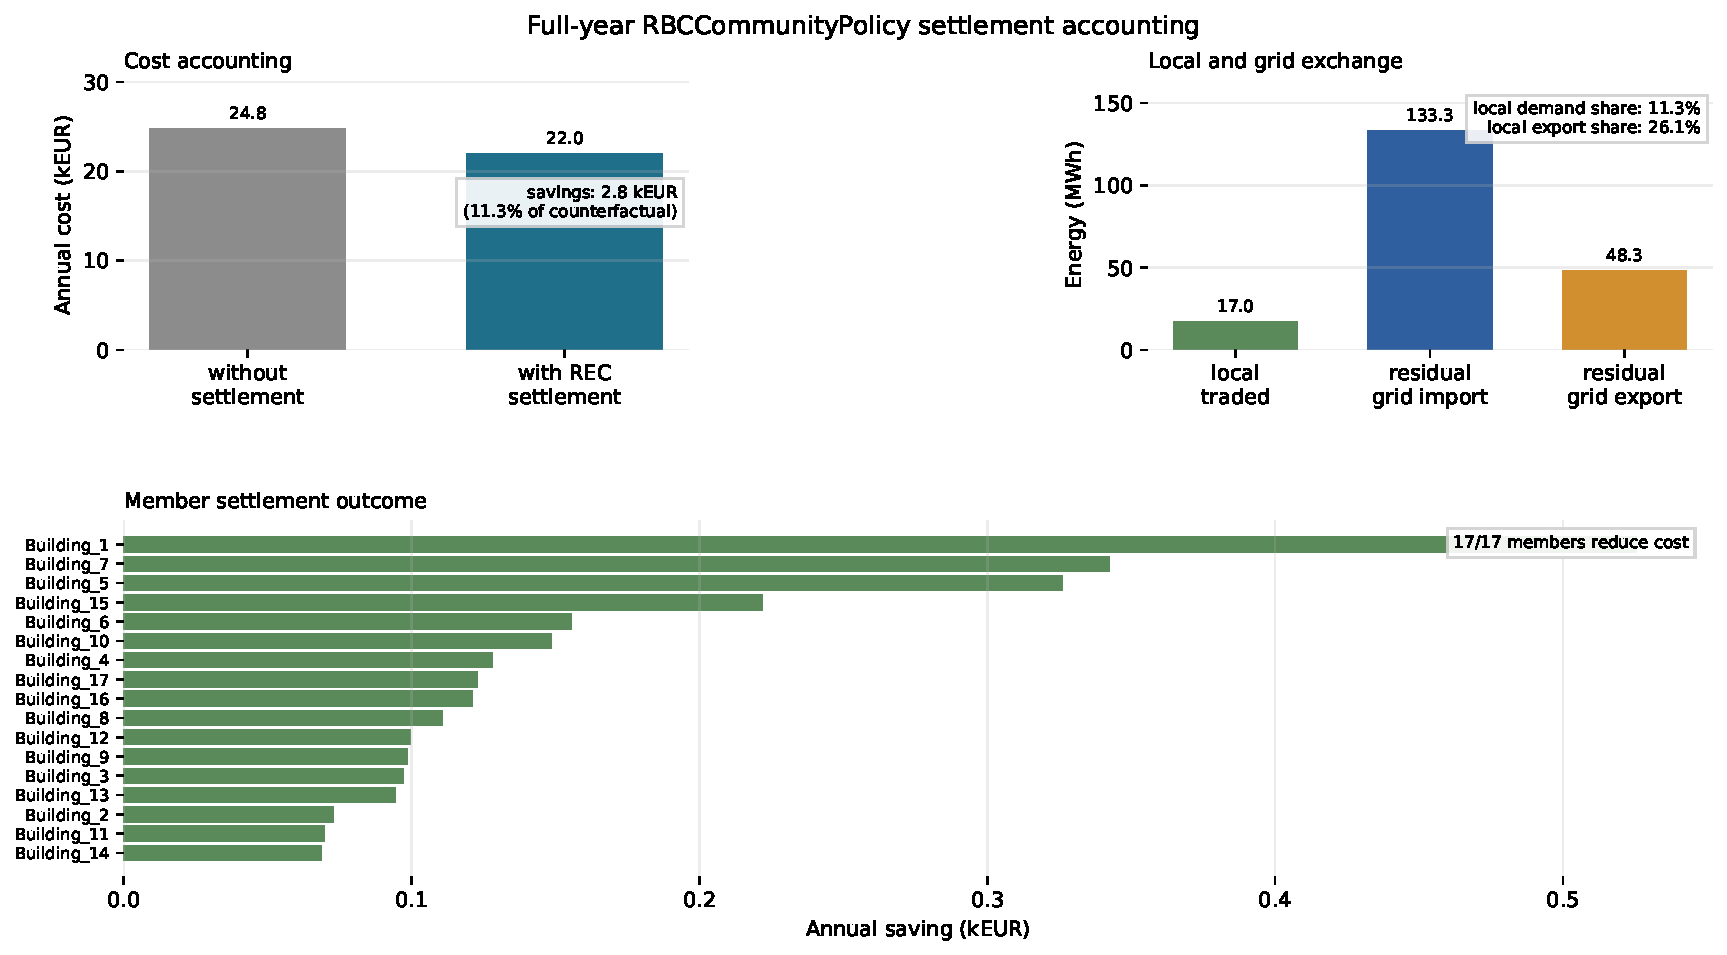
\includegraphics[width=0.96\textwidth]{simulator-rec-settlement.pdf}
\caption{\gls{rec} and participant outcomes under two accounting rules for the same historical trajectory.}
\label{fig:sim-rec-settlement}
\end{figure}

\gls{dr} introduces a service requested from outside the \gls{rec}. Each request declares its issuer, direction, interval, target power, tolerance, remuneration, penalty, and reference method. Keeping the request explicit distinguishes service delivery from an ordinary response to price. For a reduction request, charging the example vehicle later can release power now, provided its departure requirement remains achievable.
\begin{samepage}
\begin{equation}
d_{r,t}=\begin{cases}P_t-B_{r,t},&\text{up request},\\B_{r,t}-P_t,&\text{down request}.
\end{cases}
\label{eq:sim-dr-delivery}
\end{equation}
Here, $r$ identifies a demand-response request, $P_t$ is \gls{rec} import power, $B_{r,t}$ is its reference power, and $d_{r,t}$ is delivered response, in kW. An up request asks for increased import, and a down request asks for reduced import; positive $d_{r,t}$ therefore denotes movement in the requested direction. Credited response is capped by the target, shortfall accounts for tolerance, and Equation~\ref{eq:sim-power-energy} converts power into interval energy for settlement.\par
\end{samepage}

\begin{samepage}
The Portugal scenarios use the native preceding-hour mean as their reference, recorded with the result. A paired run with the same controller and no activation measures the change caused by the request. This separates contractual accounting from additional response; Section~\ref{sec:sim-evaluation} also retains rebound and terminal stored energy in the comparison.\par
\end{samepage}

\subsection{Changing Participation and Operating Conditions}
\label{sec:sim-events}
\label{sec:sim-interfaces}

A \gls{rec} can acquire a charger, lose a participant, or encounter a temporary equipment failure. Scenario events specify when these changes occur and which identities they affect. Membership and asset events are resolved before the controller acts, so state progression, observations, actions, settlement, and evaluation use the same active collection.

A removed member retains its earlier records and leaves subsequent \gls{rec} accounting. A newly installed charger contributes observations, actions, and service obligations from its activation. Stateful assets use their declared boundary state when associated with the runtime, and historical records preserve earlier instances. The configuration determines whether an event represents temporary availability or a permanent change in the \gls{rec}. Section~\ref{sec:sim-dataset-variants} explains the permanent histories selected for the Portugal collection.

Figure~\ref{fig:sim-dynamic-topology} follows one such sequence through the implementation. A member joins at step 1000, a charger is added at 1300, another charger is removed at 1500, and \gls{pv} equipment is removed at 1600. The structured observations and action rows follow the resulting resource collection. This is the setting required to study scalability under changing composition: the later control methods must encounter the updated resources, and their results must remain associated with the services active at each time \parencite{fonseca2026citylearnv3}.

\begin{figure}[htbp]
\centering
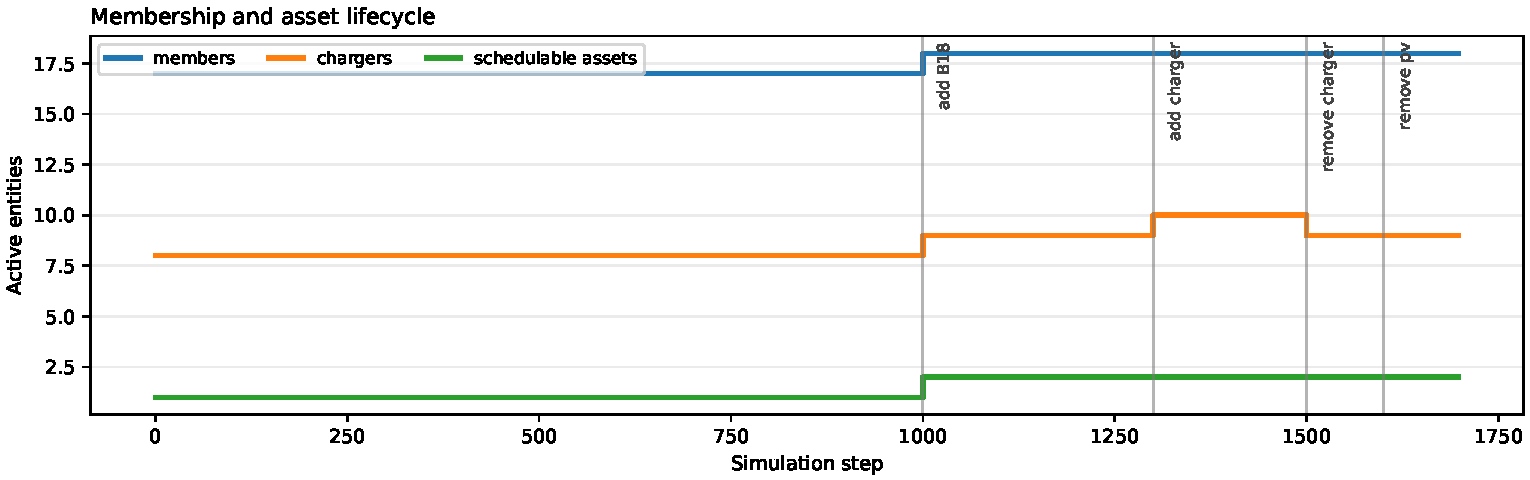
\includegraphics[width=0.96\textwidth]{simulator-dynamic-topology.pdf}
\caption{Propagation of membership and equipment events through the simulated resource collection.}
\label{fig:sim-dynamic-topology}
\label{fig:sim-topology-timeline}
\end{figure}

\begin{samepage}
Robustness requires a further experimental capability. The same \gls{rec} must be able to encounter a specified failure while retaining the underlying demand, resources, and service requests of its nominal comparison. For the example vehicle, a missing state-of-charge reading and a lost charging command are different problems: one changes the information available to decide, while the other changes the effect of the decision.\par
\end{samepage}

Failures act at different points in the same decision loop. A missing measurement changes the information supplied to a policy; a biased forecast changes an expectation; a delayed or lost command changes actuation; and unavailable equipment restricts the feasible resource set. Their effect can be expressed through separate transformations:
\begin{samepage}
\begin{equation}
\begin{aligned}
\tilde{o}_t&=\rho_o(o_t,\mathcal{E}^{o}_t,\mathcal{E}^{u}_t),&
\tilde{f}_t&=\rho_f(f_t,\mathcal{E}^{f}_t),\\
a_t^{\mathrm{cmd}}&=\rho_a(a_t^{\mathrm{req}},\mathcal{E}^{a}_t),&
a_t^{\mathrm{app}}&=\Gamma(a_t^{\mathrm{cmd}},x_t,e_t).
\end{aligned}
\label{eq:sim-robustness-channels}
\end{equation}
Here, $o_t$ and $f_t$ are nominal observations and forecasts, and their tilded forms are the values exposed after perturbation. The event sets $\mathcal{E}^{o}_t$, $\mathcal{E}^{f}_t$, $\mathcal{E}^{a}_t$, and $\mathcal{E}^{u}_t$ describe observation, forecast, command, and availability failures. Functions $\rho_o$, $\rho_f$, and $\rho_a$ apply their configured transformations. The intermediate command $a_t^{\mathrm{cmd}}$ is the request after command disturbance, while $\Gamma$ denotes the remaining action handling, including resource availability, used to obtain $a_t^{\mathrm{app}}$. These expressions identify the failure channels; their configured order is retained with the scenario.\par
\end{samepage}

Separate event streams make each failure channel an experimental variable. A missing observation can first be studied with working equipment, then combined with a lost command to examine their interaction. Noise, bias, stuck values, clipping, delay, dropout, and equipment unavailability specify different disturbances; seeds make stochastic perturbations repeatable. The nominal demand and service requests remain common to the paired runs, so changes in their outcomes can be related to the imposed disturbance.

Figure~\ref{fig:sim-robustness-channels} illustrates the resulting separation in a diagnostic run. Missing observations, forecast bias, command dropout, and equipment unavailability occupy different windows. The exported trajectory retains the nominal information, the information exposed to the controller, and the requested and applied actions. Later robustness comparisons can consequently measure service loss and recovery under a reproducible disturbance and examine which part of the control loop was affected \parencite{fonseca2026citylearnv3}.

\begin{figure}[H]
\centering
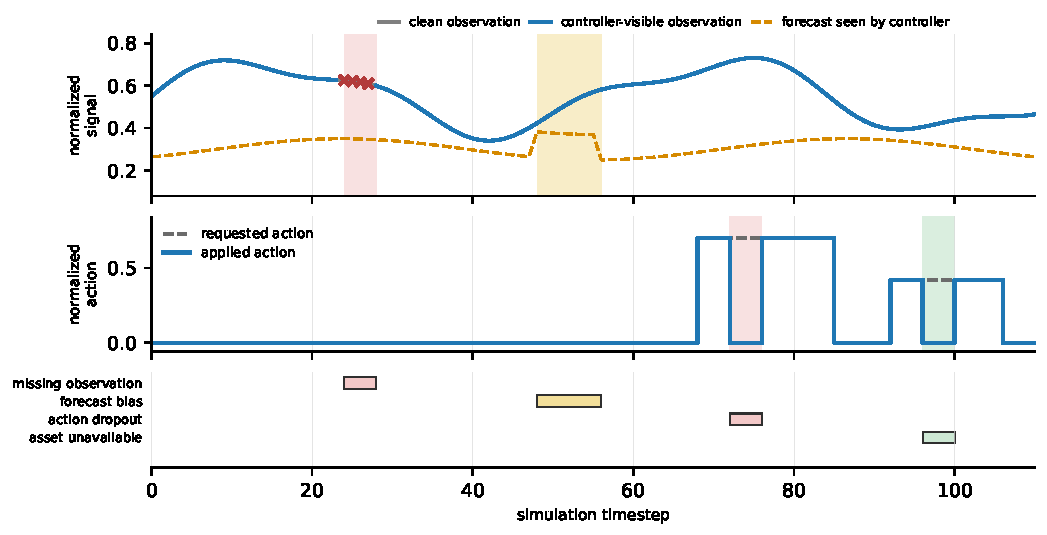
\includegraphics[width=0.96\textwidth]{simulator-robustness-channels.pdf}
\caption{Separate observation, forecast, command, and equipment-availability disturbances in the diagnostic run.}
\label{fig:sim-robustness-channels}
\end{figure}

\subsection{Controller Interfaces and Multiple Communities}
\label{sec:sim-entity}

The interaction follows the familiar reset-and-step sequence: initialise an episode, receive an observation, submit an action, and obtain the next observation, reward, and diagnostic information. A flat interface supports methods expecting fixed arrays. A structured interface organises data by entity type, identifier, relationship, availability, and action bounds. When a charger is installed, its row identifies the resource and its building instead of leaving its meaning dependent only on a vector position.

Both views use the same resource models and scenario events. This allows experiments to examine the effect of controller representation while keeping the physical setting common. Existing methods can use a compatible fixed view, while set- and graph-based methods can process active resource collections. Chapter~\ref{chap:ti-marl} develops the typed representation used for changing local interfaces. Resource identities, observation fields, and action bounds also supply the input/output description exported with the model in Chapter~\ref{chap:energAIze}, connecting simulated evaluation to deployment.

Several \glspl{rec} can be simulated together through \texttt{MultiCommunityEnv}. Each has its own scenario, buildings, controller, rewards, and outcomes, with a common clock advancing them in lockstep. Synchronised runs share the timestep, episode length, and compatible interface settings. This permits population and portfolio studies to measure local performance alongside the combined computational workload. Exchange between \glspl{rec} is a separate scenario choice; the aggregation rules in Section~\ref{sec:sim-scorecard-aggregation} combine their results without altering their physical trajectories.

\label{sec:sim-validation}
The implementation was examined through regression tests, physical and time-unit checks, controller-interface checks, and consistency checks on indicators and exports. The simulator study documents these procedures, their outcomes, and computational measurements \parencite{fonseca2026citylearnv3}; Appendix~\ref{app:simulator-audit-evidence} retains the supporting records. The figures above draw on its archived examples and show the implemented mechanisms that the datasets and controller comparisons below use.

\section{Community Datasets and Experimental Scenarios}
\label{sec:sim-annual-dataset-suite}

The datasets turn the capabilities described above into a progression of experimental settings. Small \glspl{rec} make individual decisions easy to inspect; larger \glspl{rec} introduce more resources, different daily routines, and concurrent service demands. Controlled scenario variants then change selected operating conditions. The Portugal collection follows this progression through four scenario bases and nine configurations, giving the later controller studies a common set of inputs whose purpose and assumptions are explicit.

The current edition covers 2023 and 2024 continuously at 15-minute resolution. It contains 70,176 records: 35,040 for 2023 and 35,136 for leap-year 2024. Two consecutive years provide different weather, prices, and routine realisations while preserving the \gls{rec} history. The collection is identified as \texttt{portugal-native-2023-2024-v3.1}; Appendix~\ref{app:portugal-current-audit} gives its descriptive analysis, audit results, and reproducibility record. Earlier annual experiments remain identified with their original datasets in Appendix~\ref{app:annual-suite-contract}.

\subsection{Construction and Common Assumptions}
\label{sec:sim-dataset-common-contract}

Public energy and weather sources provide the external chronology, while synthetic members and routines supply heterogeneous \gls{rec} activity. Portuguese demand statistics and E-REDES profiles inform consumption levels and shapes; household presence, opening hours, and simplified end uses introduce variation between members \parencite{dgegconsumption2023,pordataconsumption2023}. \gls{pv} production follows the site's geometry and installed equipment using the archived solar resource. \gls{omie} supplies the wholesale price chronology, and the reference tariff adds the declared variable components. Weather and carbon inputs retain their own sources and derivations, documented in Appendix~\ref{app:portugal-current-audit}.

The \gls{utc} timeline preserves elapsed time through daylight-saving changes. Civil-time fields in \texttt{Europe/Lisbon} preserve the meaning of arrivals, opening hours, holidays, and school calendars. This matters for the running example: an 08:00 departure is a local service requirement, while the energy delivered depends on the number and duration of physical intervals before it.

The second year preserves the members and equipment and continues the composition reached at the end of 2023. Permanent departures and retirements remain effective. New weather, market data, and deterministic realisations of routines supply another year of operating conditions. Sessions crossing New Year retain their continuity, so midnight does not create an artificial vehicle arrival. A simulation beginning partway through this history must initialise the corresponding topology and resource state.

Prices use one common \gls{btn} bi-hourly indexed reference across all members. The stored series contains the full variable purchase price; export to the grid is unremunerated. Local exchange is disabled in the distributed data schemas and can be enabled in the resolved experiment configuration at 80\% of the common grid-purchase price. This keeps the price convention explicit while preserving differences in the members' electrical connections and equipment.

Forecast inputs distinguish information already available from later realisations. Price forecasts use published day-ahead information when available and persistence otherwise; weather uses daily persistence. The corresponding forecast errors and publication boundary are analysed in the appendix. These simple references provide a reproducible information setting for the controller comparisons.

\subsection{Community Bases and Their Experimental Roles}
\label{sec:sim-dataset-composition}

The four bases offer different ways of examining controller behaviour. Table~\ref{tab:sim-annual-suite-composition} gives their complete inventories; the differences in ownership and activity explain the experimental role of each one.

\paragraph{Core-4: inspectable local decisions.}
Four residential members form a compact \gls{rec} with one \gls{pv} site, one stationary battery, and two charging sites. This makes it possible to follow a decision from one resource to the \gls{rec} balance. The evening charging example can be inspected alongside a neighbour's solar production or a battery schedule, and a missed departure can be traced back through the preceding actions. Core-4 is consequently useful when establishing that a controller receives the intended information and delivers the expected services before undertaking more expensive studies.

\paragraph{Core-15: residential diversity and method development.}
Fifteen households introduce more combinations of generation, charging, appliance use, and consumption-only participation. Different routines make flexibility available at different times even though the setting remains residential. This supports method development, reward and observation studies, and repeated comparisons of candidate designs at a moderate computational cost. Overlapping arrivals and appliance windows make several households compete for favourable periods. The controller must use differences in their available time while maintaining each service.

\paragraph{Core-30: mixed activity and controlled comparisons.}
Twenty-four households and six service premises extend demand and charging activity across the day. Ten \gls{pv} sites, three stationary batteries, fifteen charging connectors, and nineteen controllable appliances create concurrent decisions under finite electrical headroom. Core-30 Normal supplies the reference \gls{rec} for the Topology, Safety, Robustness, and Combined configurations. Daytime service activity changes the demand available to absorb solar production, while residential charging extends obligations into the evening. Keeping this physical base common across variants isolates the operating condition being studied.

\paragraph{Premium-100: larger and more heterogeneous communities.}
Eighty households and twenty service premises include offices, retail, clinics, cafes, workshops, and facilities with longer operating hours. The complete base contains twenty batteries and sixty-five charging connectors; one office has twelve ports. Premium Normal supports studies of larger populations and richer local interfaces, while Premium All-in combines changing participation with disturbances and demand-response services. The concentration of chargers at individual sites creates a further scheduling difficulty: several departures can compete for one building's electrical headroom. The scalability study therefore concerns both \gls{rec} size and the number of decisions within a member.

\begin{table}[!htbp]
\centering\small
\caption{Complete physical inventories in the Portugal 2023--2024 collection.}
\label{tab:sim-annual-suite-composition}
\begin{tabularx}{\textwidth}{@{}Xrrrr@{}}
\toprule
\textbf{Quantity} & \textbf{Core-4} & \textbf{Core-15} & \textbf{Core-30} & \textbf{Premium-100}\\
\midrule
Members & 4 & 15 & 30 & 100\\
\gls{pv} sites & 1 & 4 & 10 & 36\\
Stationary batteries & 1 & 1 & 3 & 20\\
Charging sites & 2 & 5 & 10 & 41\\
Charging connectors & 2 & 6 & 15 & 65\\
Vehicle identities & 2 & 6 & 19 & 85\\
Controllable appliances & 2 & 10 & 19 & 64\\
Consumption-only members & 1 & 5 & 10 & 32\\
\bottomrule
\end{tabularx}
\end{table}

Ownership overlaps across all four bases. A household may produce \gls{pv} energy without owning a battery, and a consumption-only member may benefit from energy supplied by another participant. The inventories therefore describe an uneven distribution of control opportunities. Population and composition both change between bases; experiments intended to isolate the effect of population size select matched compositions in addition to reporting the base used.

A charging site, a physical connector, a vehicle identity, and a visit remain separate quantities. The two-year static catalogues contain 9,691 sessions in Core-30 and 41,288 in Premium-100, including visits censored at the record boundaries. Residential visits include commuting, night work, and daytime presence; services introduce shorter and repeated visits. Requested departure \gls{soc} ranges from 50\% to 100\%. The catalogue therefore extends the evening-arrival example into a wider range of service windows.

Controllable appliance counts refer to physical devices. Programme profiles and requests are counted separately, while fixed appliance demand is already included in the non-shiftable load. The appendix retains both quantities, together with programme energy and the time available to schedule each request.

\begin{figure}[H]
\centering
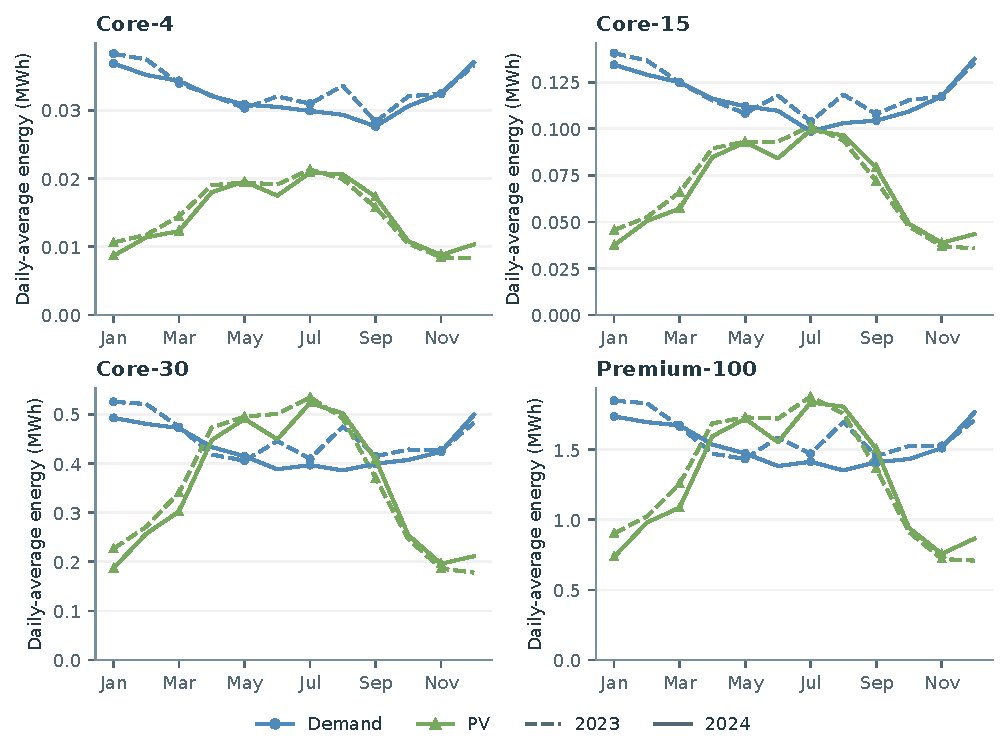
\includegraphics[width=\textwidth]{simulator-portugal-seasonal.pdf}
\caption{Monthly daily-average input demand and \gls{pv} production in the four static \gls{rec} bases.}
\label{fig:sim-dataset-profiles}
\end{figure}

Figure~\ref{fig:sim-dataset-profiles} shows the seasonal setting for these decisions. In Premium-100, non-shiftable input demand changes from 583.81 to 560.19~MWh between 2023 and 2024, and \gls{pv} production changes from 476.60 to 469.16~MWh. Within a year, the balance also changes with the season. A controller consequently encounters different opportunities for solar use even when the installed equipment is unchanged.

The daily profiles in Figure~\ref{fig:sim-dataset-daily} show the timing more directly for Core-30. The winter demand peak occurs in the evening, after \gls{pv} production has fallen, while the summer mean profile has a pronounced daytime solar surplus over non-shiftable demand. Residential vehicle presence is greatest overnight; service vehicles provide charging opportunities during the day. The controller must fit charging into these different windows while meeting departure requirements. The current connectors permit charging only, so stationary batteries provide the stored-energy flexibility between periods of production and later demand.

\begin{figure}[H]
\centering
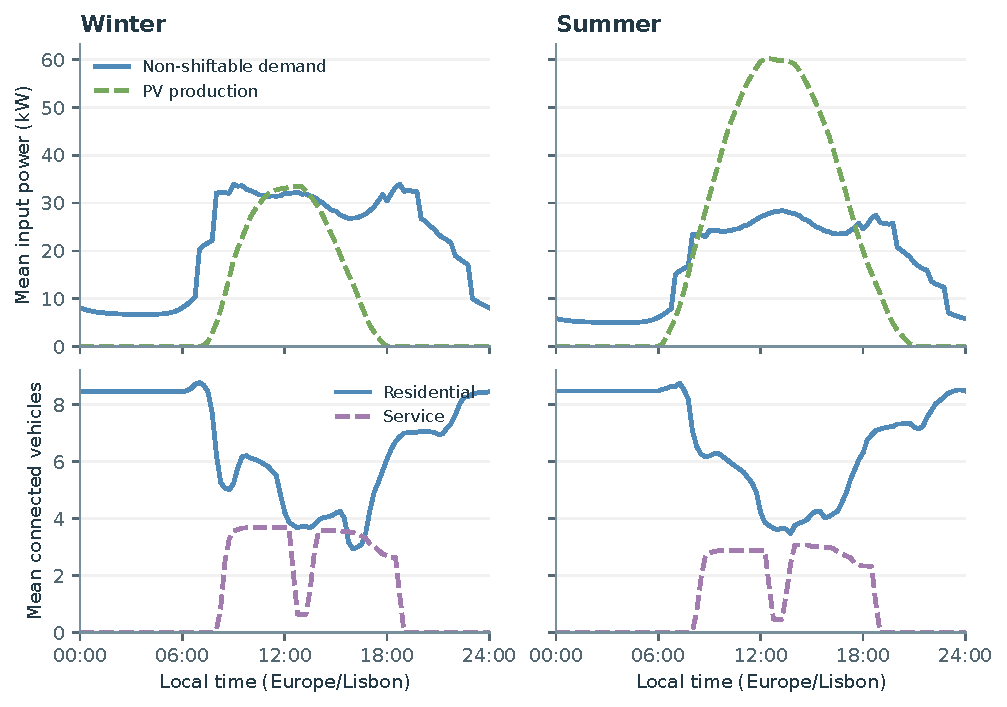
\includegraphics[width=\textwidth]{simulator-portugal-daily.pdf}
\caption{Core-30 daily input and vehicle-presence profiles: Monday--Friday means in winter (December--February) and summer (June--August) of 2024, in Lisbon local time.}
\label{fig:sim-dataset-daily}
\end{figure}

\subsection{Scenario Variants and the Questions They Address}
\label{sec:sim-dataset-variants}

The configurations distinguish the \gls{rec} being studied from the condition applied to it. The Normal cases retain the complete membership and equipment catalogue without the additional event campaigns. They establish how a controller operates with the resources, services, and electrical limits of that base. The remaining configurations make selected difficulties explicit, as summarised in Table~\ref{tab:sim-scenario-purpose}.

\begin{table}[!htbp]
\centering\small
\caption{Purpose of the scenario variants and their reference comparisons.}
\label{tab:sim-scenario-purpose}
\begin{tabularx}{\textwidth}{@{}p{0.18\textwidth}p{0.34\textwidth}X@{}}
\toprule
\textbf{Configuration} & \textbf{Change relative to its Normal base} & \textbf{Question supported}\\
\midrule
Core-30 Topology & Permanent member and equipment additions, removals, and replacements. & Can control continue as the active resource collection changes?\\
Core-30 Safety & Tighter selected building and phase limits. & Can the controller deliver services under reduced headroom, and how much action correction is needed?\\
Core-30 Robustness & Data and equipment events, observation noise, and grid interruptions. & How do disturbances affect decisions, service, and recovery?\\
Core-30 Combined & Membership changes, electrical stress, health events, and interruptions. & What happens when these conditions occur in the same \gls{rec} history?\\
Premium All-in & Participation changes, failures, interruptions, seasonal noise, and demand-response requests. & How does control perform when a larger, heterogeneous \gls{rec} faces several operating demands?\\
\bottomrule
\end{tabularx}
\end{table}

Safety changes the headroom against which actions are evaluated, making service delivery and reliance on limiting central to the comparison. Robustness retains a reproducible failure schedule, allowing nominal and disturbed trajectories to be compared through the affected services and recovery period. Topology changes which members and assets are active. These configurations give the corresponding \glspl{rq} concrete experimental contrasts. Combined and All-in then examine their interaction within an integrated workload; paired diagnostic replays can distinguish individual effects when needed.

The topology histories describe permanent participation changes. Core-30 Topology and Combined begin with 26 active members and finish with 27; Premium All-in begins with 80 and finishes with 88. The full catalogues contain the resources available to those histories. Events also install, replace, or retire equipment. A member that leaves exits subsequent \gls{rec} demand and service accounting, and the same departure is not replayed in 2024.

Failure events and observation noise remain separate scenario settings. The former specify intervals of missing data, forecast bias, delayed or lost commands, and equipment unavailability. Core-30 Robustness additionally includes its continuous measurement-noise setting, while Premium All-in uses seasonal noise campaigns. Backup during grid interruptions follows the aggregate convention supported by the selected runtime. The timing and intensity of these conditions remain explicit, allowing service loss and recovery to be evaluated against matched nominal operation.

\gls{dr} appears only in Premium All-in. Each year includes two one-hour reduction requests of 80~kW and one one-hour absorption request of 40~kW, together with a separately identified four-hour reduction request of 1500~kW. The last is a deliberately excessive request used to examine behaviour under unattainable service demand. Its outcome belongs to a separate stress category from the operational candidate requests.

Development and reserved confirmation files select different event schedules within these configurations. A paired comparison retains the physical inputs and declares the event or operating condition changed. The two-year chronology also permits temporal separation, with training, selection, and confirmation windows specified by each controller study. Initialisation preserves the \gls{rec} history at the selected start time, so a member that departed earlier remains absent.

\subsection{Data Characterisation and Quality}
\label{sec:sim-annual-baseline-audit}

The dataset analysis follows the same distinctions used in construction: installed and active resources, input energy and controlled energy, scheduled visits and delivered charging, and requested services and completed services. Appendix~\ref{app:portugal-current-audit} develops that analysis through distributions, temporal profiles, and event summaries. It also records the checks supporting the current edition.

The input checks cover the time axis, calendar, inventories, resource identities, connection schedules, appliance windows, forecasts, and event histories. Individual charging requests are also examined against their connection duration, accepted power, losses, and battery taper. The resulting audit accompanies the descriptive analysis in the appendix. Concurrent demand, electrical limits, disturbances, and the controller's decisions then determine which services are delivered during simulation.

The archived examples in Section~\ref{sec:sim-architecture} illustrate the implemented mechanisms. The Portugal collection supplies the inputs for the controller comparisons that follow, with its descriptive analysis and audit retained together in the appendix.

\section{Performance Indicators and Evaluation Protocol}
\label{sec:sim-evaluation}

The value of a control decision depends on the service it delivers and the resources it uses. Returning to the example vehicle, a lower electricity bill is useful when the vehicle is ready at 08:00 and the charging schedule respects the installation limits. A \gls{rec} assessment must also show whether the gain is shared among its members and how the controller behaves when conditions change. The evaluation therefore reads energy and economic outcomes together with service, safety, robustness, and computational effort.

The simulator extends the inherited energy indicators with participant services, local settlement, electrical constraints, and operating events. The definitions below establish the common scorecard and comparison rules used in the following chapters. Scenario choice determines the members, resources, prices, and active services; Chapters~\ref{chap:control-benchmark} and~\ref{chap:ti-marl} specify the learning methods, training budgets, data windows, seeds, and ablations. Each result is thus read against the same definitions while retaining the conditions of its experiment.

\subsection{Energy, Cost, and Community Outcomes}

Grid import and export record how much energy crosses the selected building or \gls{rec} boundary. Their difference is net exchange, but the two directions remain available separately: identical net totals can arise from very different patterns of consumption and surplus. Local sharing records which part of member demand is met within the \gls{rec} and how the associated payments are allocated. The accounting boundary and settlement settings are consequently part of every comparison.

For a matched reference controller, cost saving is
\begin{samepage}
\begin{equation}
\Delta C=C_{\mathrm{ref}}-C_{\pi}.
\label{eq:sim-cost-saving}
\end{equation}
Here, $C_{\pi}$ is the cost of the evaluated policy $\pi$, and $C_{\mathrm{ref}}$ is reference cost over the same members, intervals, prices, and settlement rules. The saving $\Delta C$ is expressed in currency and is positive when the evaluated policy reduces cost. Demand-response payments and penalties remain identifiable within the reported cost after settlement. Absolute savings also remain interpretable when the reference cost is zero or negative.\par
\end{samepage}

Participant outcomes extend this reading beyond the \gls{rec} sum. The savings count includes members active in the scored period with finite costs in both runs; a member saves when its cost difference is positive. The scorecard gives this count, its percentage of eligible members, and the distribution of absolute savings. Percentage cost reductions additionally require a positive reference cost. In a changing \gls{rec}, each member is compared over its active period. Figure~\ref{fig:sim-rec-settlement} shows why this matters: the same sharing mechanism produces different benefits for members with different generation and demand.

Solar self-consumption relates generation to the amount retained within the stated accounting boundary:
\begin{samepage}
\begin{equation}
S_{\mathrm{PV}}=100\frac{G-X_{\mathrm{PV}}}{G},\qquad G>0.
\label{eq:sim-solar-use}
\end{equation}
Here, $G$ is total \gls{pv} generation and $X_{\mathrm{PV}}$ is the energy attributed to \gls{pv} export at that boundary, both in kWh. The indicator $S_{\mathrm{PV}}$ is a percentage; it is undefined when there is no generation. Building and \gls{rec} values refer to different boundaries, since energy exported by one member may be consumed by another. The source totals accompany the ratio so that the level of aggregation remains clear.\par
\end{samepage}

Battery throughput sums the charging and discharging energy of stationary batteries at the declared metering boundary, in kWh. \gls{v2g} export separately totals the energy supplied by vehicle batteries, also in kWh. Their interpretation depends on the cost, service, and grid outcomes achieved, together with any degradation model included in the experiment. A larger throughput can accompany useful solar shifting or unnecessary cycling; its magnitude explains resource use without supplying an independent ranking.

Operational emissions accumulate imported electricity multiplied by the corresponding interval carbon intensity, giving kg~CO$_2$. The report identifies whether imports are measured at individual member meters or after \gls{rec} balancing, and uses the same boundary for all methods. Any export credit follows an explicitly declared accounting rule. These quantities allow two equally inexpensive schedules to be distinguished by renewable utilisation, storage use, or emissions.

The grid-shape indicators use \gls{rec} net power, positive for import. The all-time peak is its maximum over the scored period. Daily peak is the mean of the maxima in successive 24-hour windows from the episode start; at 15-minute resolution, each complete window contains 96 intervals. A final partial window is included when present. The daily load-factor penalty averages one minus the ratio of mean to maximum power in those windows. Raw peaks are in kW, while the load-factor penalty is dimensionless. The scorecard reports both peaks in kW; the load-factor penalty remains available in the wider catalogue.

Ramping uses the sum of positive changes in \gls{rec} net power between consecutive intervals, including intervals of net export. It therefore measures upward changes, such as the rise when evening charging begins as solar production falls. The scorecard reports this accumulated upward change in kW over the complete evaluation window. It is a sum of power increments, rather than a rate in kW per hour. These conventions follow the simulator's power-based comparison outputs. Legacy indicators calculated from interval energy retain their separate units; comparisons use the same resolution and convention throughout.

\subsection{Service Delivery, Safety, and Robustness}
\label{sec:sim-service-evaluation}

Vehicle service is evaluated at departure with a tolerance of five percentage points of \gls{soc}. Minimum acceptable service is reached at or above the requested target minus this tolerance. Target accuracy requires the final state to lie within five percentage points on either side of the target. For an 80\% request, minimum service begins at 75\%, while the accuracy band is 75--85\%. The corresponding rates are
\begin{samepage}
\begin{equation}
S_{\min}=100\frac{N_{\min}^{\mathrm{met}}}{N_{\min}^{\mathrm{eligible}}},\qquad
S_{\mathrm{tol}}=100\frac{N_{\mathrm{tol}}^{\mathrm{met}}}{N_{\mathrm{tol}}^{\mathrm{eligible}}}.
\label{eq:sim-service-rates}
\end{equation}
Here, $S_{\min}$ and $S_{\mathrm{tol}}$ are the minimum-service and within-tolerance percentages. For each criterion, $N^{\mathrm{eligible}}$ counts eligible departures and $N^{\mathrm{met}}$ counts those meeting the criterion. A rate is undefined when its eligible count is zero. The counts and the number of excluded departures accompany both percentages.\par
\end{samepage}

An eligible departure has an observed session end, a valid target and achieved \gls{soc}, and a threshold reachable under the simulator's maximum-charge feasibility screen. This screen starts from the session boundary state and follows the available connection intervals, charger and battery power limits, efficiencies, and battery taper. It applies the configured electrical headroom and outage handling. Eligibility is calculated for each threshold, independently of whether the controller meets it. The common five-point tolerances give both criteria the same lower threshold; their success counts differ when charging exceeds the upper accuracy limit. Individually unattainable requests remain visible alongside the eligible results.

The service record gives failed departures as a count over eligible departures and reports both the total and largest individual energy deficit. For each eligible departure, the deficit is the positive difference between the battery energy required at the minimum-service threshold and the energy present at departure, in kWh. This distinguishes many small shortfalls from a few severely underserved vehicles. Energy missing from the original requested target remains a separate diagnostic, since the minimum-service criterion includes the stated tolerance. Unattainable requests and exclusions caused by missing or incomplete records retain separate counts. A paired disturbance comparison also identifies departures that lose eligibility and reports service on the common eligible cohort, so that an outage cannot improve the apparent rate simply by removing difficult requests.

Appliance service is read through completed and missed cycles, completion deadlines, start delay, delivered energy, and unserved energy. A shifted washing programme can then be distinguished from a programme that never ran. Demand-response records likewise retain requested and credited response, shortfall, compliance, and settlement for each activation. These service quantities remain visible beside energy savings, including in Combined and All-in scenarios where several obligations compete for the same flexibility.

Electrical safety is measured on the applied trajectory, while requested pressure describes the actions proposed before limiting. Accumulated exceedance can be written as
\begin{samepage}
\begin{equation}
V=\frac{\Delta t}{3600}\sum_{t\in\mathcal{T}}\sum_{\ell\in\mathcal{L}_t}
\left([P_{\ell,t}-I_{\ell}^{\max}]_+ +[-P_{\ell,t}-X_{\ell}^{\max}]_+\right).
\label{eq:sim-violation-energy}
\end{equation}
Here, $\mathcal{T}$ contains the scored timesteps and $\mathcal{L}_t$ the configured total-building and phase boundaries active at timestep $t$. Applied power $P_{\ell,t}$ is positive for import; $I_{\ell}^{\max}$ and $X_{\ell}^{\max}$ are positive import and export limits, all in kW. The notation $[z]_+=\max(z,0)$ retains positive excess, and $\Delta t$ is the timestep in seconds. Thus, $V$ measures accumulated constraint exceedance in kWh, counting each violated total or phase limit. The residual calculation uses a numerical tolerance of $10^{-5}$~kW.\par
\end{samepage}

The frequency of actual action corrections accompanies this applied safety result:
\begin{samepage}
\begin{equation}
 A_{\mathrm{corr}}=100\frac{N_{\mathrm{corr}}}{N_{\mathrm{decision}}}.
 \label{eq:sim-action-correction}
\end{equation}
Here, $N_{\mathrm{decision}}$ counts eligible building-level decision opportunities with an active controllable resource and a supplied proposal. The numerator $N_{\mathrm{corr}}$ counts those opportunities in which at least one command is actually changed by the declared feasibility or supervisory stages. The rate $A_{\mathrm{corr}}$ is a percentage, with a stated numerical tolerance for detecting changes. Each building decision is counted once even if several commands or stages change it.\par
\end{samepage}

A call to a validator with an unchanged output adds no correction. Missing, invalid, or late decisions are counted once per building decision opportunity when a usable action is unavailable by the declared control deadline. Their denominator includes all opportunities requiring a decision, including those with no proposal. This differs from the correction denominator, which requires a supplied proposal. The report names the stages included and preserves proposed, submitted, and applied actions, following Section~\ref{sec:sim-contracts}.

Fallback records describe the supervisor's response. An episode is a consecutive period of fallback within one building; separate buildings contribute separate episodes. Total duration is summed in building-minutes, with overlapping periods therefore retained for each affected building. Per-resource corrections and their magnitude remain available for diagnosis. A corrected command or a fallback decision can preserve the requested service, so intervention and missed service keep separate counts. Injected fault episodes and their duration describe exposure to the disturbance and are recorded independently of these outcomes.

Robustness uses the same outcomes in paired nominal and disturbed runs. The comparison fixes the underlying scenario, controller, and random seeds and changes the selected disturbance. It reports energy and cost differences, missed or delayed services, and action correction during the event and afterwards. Execution recovery is measured from clearance of the declared external fault to the first usable controller decision applied within its deadline. Median and maximum recovery time accompany the number of recovered and unrecovered episodes. Episodes still unresolved at the observation boundary retain their elapsed duration as a lower bound. Service recovery is reported separately where an obligation can still be fulfilled; a missed departure remains a missed service even after timely execution resumes.

\subsection{Scorecard, References, and Aggregation}
\label{sec:sim-scorecard-aggregation}

The simulator provides a much wider set of performance indicators than can be usefully displayed in every comparison. Member savings use matched \gls{bau} operation as a reference, with its storage variants defined in Chapter~\ref{chap:control-benchmark}. The common scorecard in Table~\ref{tab:sim-core-scorecard} selects fifteen indicators that keep the results aligned across methods, datasets, and chapters. It gives an economic outcome its energy, service, and operational context. The wider catalogue in Appendix~\ref{app:sim-kpi-catalogue} remains available for questions about appliance service, local settlement, \gls{dr}, topology, failures, comfort, degradation, and multi-\gls{rec} operation.

\begin{table}[!htbp]
\centering
\caption{Common scorecard. Physical and monetary quantities retain their absolute units; percentages describe service, utilisation, or intervention directly.}
\label{tab:sim-core-scorecard}
\footnotesize
\setlength{\tabcolsep}{4pt}
\renewcommand{\arraystretch}{1.16}
\begin{tabularx}{\textwidth}{@{}>{\raggedright\arraybackslash}p{0.16\textwidth}>{\raggedright\arraybackslash}X >{\raggedright\arraybackslash}p{0.25\textwidth}@{}}
\toprule
\textbf{Category} & \textbf{Indicators and units} & \textbf{Reading} \\
\midrule
Economy & \gls{rec} cost [EUR]. & Lower, with service retained. \\
Emissions & Operational emissions [kg CO$_2$]. & Lower under the same accounting rule. \\
Energy & External \gls{rec} import [kWh]; external \gls{rec} export [kWh]; solar self-consumption [\%]. & Read the two exchange directions with local solar use. \\
Grid shape & Mean daily peak [kW]; maximum peak [kW]; accumulated upward ramping [kW]. & Lower under matched service and timestep. \\
\gls{ev} service & Minimum service [\%]; target accuracy [\%, $\pm5$ \gls{soc} percentage points]. & Retain the eligible and excluded departure counts. \\
Safety and supervision & Electrical violations [kWh]; actual action corrections [\% of eligible building decisions]. & Zero residual violation; interpret correction with delivered service. \\
Resource use & Stationary-battery throughput [kWh]; \gls{v2g} export [kWh]. & Explain how flexibility was used. \\
Member benefit & Members saving against matched \gls{bau} [$n/N$]. & Show the distribution of \gls{rec} benefit. \\
\bottomrule
\end{tabularx}
\end{table}

Results use the same names and units throughout the thesis. Cost is the \gls{rec} total under the declared tariff and settlement convention; savings in EUR may accompany it. Grid import and export are measured at the \gls{rec} boundary, while the sum of member-meter imports is retained separately where useful. Service and self-consumption percentages keep their direct meaning: they express fulfilled departures or retained generation, rather than normalisation against another controller. The principal tables report cost, energy, emissions, and power in absolute units. Reference differences support interpretation without replacing those quantities.

The common operating reference uses ordinary vehicle charging, execution of mandatory appliance requests, and simple \gls{pv} self-consumption storage. A no-storage variant isolates the contribution of enabling that resource. Progressively informed \glspl{rbc} use prices, generation, peaks, and \gls{rec} information. Chapter~\ref{chap:control-benchmark} develops these references alongside optimisation and learning. Member benefit uses the matched storage-enabled \gls{bau} unless another reference is explicitly named; an incremental hierarchy comparison can additionally report savings against the same local controller without coordination.

The scorecard can be presented in two blocks with the same method order: economy, emissions, energy, and grid shape first; service, safety, resource use, and member benefit second. A focused comparison can select the methods and columns relevant to its question. A charging study, for example, may place cost beside the two \gls{ev}-service rates and intervention, while a coordination study also needs the \gls{rec} power profile and member outcomes. Safety and disturbance studies add a compact service-and-event table: failed obligations, their energy deficit, unavailable decisions, fallback, and recovery. Each table retains its dataset, complete evaluation window, and indicator definitions, allowing the comparisons to accumulate as the methods are introduced.

Additional indicators follow the services present in the experiment. A dataset containing deferrable appliances requires completion and missed-deadline outcomes beside the energy comparison; demand-response experiments retain delivered response, shortfall, and settlement. A disabled service is identified as such. Unavailable measurements remain marked as unavailable, rather than filled with a favourable zero. Export and battery throughput are diagnostic quantities, and a high value alone does not establish better control.

These observations connect directly to the four research dimensions established in Chapter~\ref{chap:introduction}. \emph{Scalability} follows control quality as the number of members and resources grows, together with training time [h], peak memory [GB], and inference latency [ms per building decision]. It also records the preparation or retraining needed after a configuration change. \emph{Deployability} concerns the work needed to place the controller in service: configuration and integration effort [person-hours], elapsed deployment time, runtime dependencies, and the successful reproduction of the evaluated decisions through the deployed inference path. Those measurements accompany the scorecard in the corresponding studies.

\emph{Safety} is read through service fulfilment, physical violations, and the interventions supporting the applied decisions. \emph{Robustness} uses the same outcomes in paired nominal and disturbed conditions, supplemented by fallback and service-specific recovery times. The common scorecard thus supplies a stable account of useful operation, while each investigation adds the observations needed to examine its \gls{rq}. Keeping these meanings stable allows the architecture, simulation, and learning studies to contribute to the same argument.

Aggregation follows the measured quantity. Cost sums the member bills under the selected settlement rule; internal payments cancel in the \gls{rec} total when transfers between members are represented. Energy and emissions accumulate over the scored intervals at their declared boundary. Solar self-consumption is calculated from total generation and \gls{pv}-attributed export, rather than the unweighted mean of building percentages. Maximum peak is taken from the aggregate \gls{rec} trajectory, mean daily peak averages its daily maxima, and ramping accumulates its successive positive power changes. None of these power quantities is obtained by summing independently computed building peaks.

Service rates pool the corresponding met and eligible event counts, and correction rates pool corrected and eligible building decisions. Their denominators and exclusions remain visible. Member benefit counts matched active members with finite bills and retains the range of absolute savings in the detailed results. Each dataset is reported separately. Where repeated training runs are available, each run first yields a scorecard for the full test window; the report then gives the mean and dispersion across independent training seeds, retaining paired simulator conditions for each comparison.

\subsection{Temporal Protocol and Reproducible Comparisons}
\label{sec:sim-temporal-protocol}

The two-year Portugal collection separates controller development from operation on a later annual sequence. The studies in Chapter~\ref{chap:control-benchmark} use 2023 for training and validation and reserve the complete available 2024 sequence for final evaluation. A full year exposes a controller to changing demand, solar production, prices, and service requirements across the seasons. Short event plots explain particular decisions within that annual account.

Training allows the agent to interact with the simulator and improve its policy. Validation evaluates selected policies on reserved periods to choose hyperparameters, reward settings, and checkpoints. Four fortnightly blocks---the first fourteen days of February, May, August, and November 2023---provide validation conditions in different seasons. The remaining 2023 intervals supply training episodes. Table~\ref{tab:sim-temporal-split} identifies the role of each partition.

\begin{table}[htbp]
\centering\small
\caption{Temporal separation for the principal controller comparisons.}
\label{tab:sim-temporal-split}
\begin{tabularx}{\textwidth}{@{}p{0.17\textwidth}p{0.33\textwidth}X@{}}
\toprule
\textbf{Stage} & \textbf{Data window} & \textbf{Use}\\
\midrule
Training & 2023, excluding the four reserved validation blocks. & Generate interaction experience, update the policy, and fit preprocessing statistics.\\
\addlinespace
Validation & Days 1--14 of February, May, August, and November 2023. & Compare configurations and select checkpoints with learning disabled.\\
\addlinespace
Final test & Complete available 2024 sequence. & Evaluate the selected policy with its parameters, preprocessing, and action-selection rule fixed.\\
\bottomrule
\end{tabularx}
\end{table}

The split follows the dataset's \gls{utc} clock. Training episodes retain contiguous time intervals; replay records and learning targets stop at the partition boundaries. Validation observations and rewards do not enter policy updates or the fitting of preprocessing statistics. Initialisation reconstructs the active resources and relevant preceding history at each episode's start, with any warm-up kept outside the score. The continuous test year then carries stored energy and unfinished services forward without daily or monthly resets.

\gls{bau} and fixed rule-based references use the same annual test window as the learned controllers. \gls{bau} can also be evaluated over the full development year to characterise conventional operation, with 2023 and 2024 reported separately. The primary comparison pairs each controller with its reference within the same scenario and year. The seven Core-30 and Premium-100 scenarios provide this principal account; Core-4 and Core-15 support development and diagnostic inspection. Comparisons across \gls{rec} sizes additionally retain their different resource compositions.

Candidate and reference share the dataset edition, active members and resources, physical inputs, service requests, prices, settlement, electrical limits, events, timestep, and scored interval list. Initial stored energy, preceding \gls{rec} history, and the handling of services crossing either boundary are also matched. Changes of membership follow the same event schedule for all methods. The record gives the first and last scored action timestamps and the executed interval count; warm-up observations and an unexecuted terminal observation contribute no artificial energy or cost. Near-boundary forecast handling follows the same convention across the comparison.

The selected checkpoint and preprocessing statistics are frozen for evaluation. A study of online adaptation declares its update rule separately and compares it under the same test conditions. Repeated training seeds reveal variation in the learned solution, while paired simulator seeds retain common disturbances for candidate and reference. Episode segmentation preserves resource state and unfinished services across the full test sequence unless resets are themselves part of the declared experiment. This prevents a series of freshly initialised short episodes from silently replacing continuous operation.

Information access and protective settings accompany each result. Local and \gls{rec}-aware methods retain their declared observation boundaries, and forecasts use the same availability convention. A perfect-information schedule is reported separately as an opportunity reference. An optimisation method evaluated through successive horizons still covers the complete test sequence, carrying state and unfinished obligations between horizons. A short mathematical solve remains a diagnostic with its own scope; simulator replay supplies the operating outcomes needed for the common scorecard.

Disturbance studies retain complete-window outcomes as well as the intervals around each event. They fix the underlying scenario, controller, and paired random conditions, then change the declared disturbance. Additional energy, missed service, intervention, and recovery can consequently be attributed to that change. Demand-response assessment likewise retains the reference estimator, credited response, penalties, and cost after settlement. A no-activation replay with the same policy measures additional response, while subsequent intervals reveal rebound and differences in stored energy. Operational candidate requests and deliberately excessive stress requests retain separate categories.

Computational comparisons identify the hardware, software, population, resource counts, observation/action sizes, interaction budget, and update budget. Training time and memory describe development; inference measurements report the declared timing boundary, batch size, warm-up, and latency distribution. The 95th-percentile latency describes the slower part of that distribution, while late decisions are counted against the actual control deadline over the complete test window. The timing boundary states whether observation preparation, inference, validation, and dispatch are included. A change of resources additionally records model reuse, rebuilding, retuning or retraining, and the associated interruption and service outcomes.

Deployment records separate person-hours of configuration and integration from elapsed time between the start of installation and the first valid applied decision. They retain the supporting services, resource mapping, preprocessing, and controller composition placed in operation. Reproduction of the evaluated behaviour is checked by replaying the same recorded inputs through the packaged controller and counting matching requested actions within a declared tolerance. Timing compliance and successful dispatch are then assessed on the complete execution path. These measurements accompany the operating scorecard and explain how readily a useful controller can be placed in service.

The experiment record preserves the data, software, controller version, evaluation conditions, and resulting trajectories through the lifecycle described in Chapter~\ref{chap:energAIze}.

\section{Chapter Summary}
\label{sec:sim-discussion}
\label{sec:sim-open}

The simulator development provides the experimental setting needed to investigate \gls{rec} control under the conditions established in the opening chapters. CityLearn v3 connects resource models and participant services to electrical limits, changing membership, local exchange, external requests, and failures. The implemented examples show how these conditions enter the simulation and remain visible in observations, actions, and outcomes. Their incorporation into the official CityLearn distribution makes the capabilities available as a reusable research contribution.

The Portugal datasets organise those capabilities into an experimental progression, from inspectable residential decisions to larger \glspl{rec} with mixed activities and interacting events. Their documented inputs and scenario purposes support matched comparisons, while the performance indicators connect energy and economic outcomes to services, constraints, participant benefits, and computational effort.

This foundation makes scalability, safety, and robustness accessible to controlled experiments through changes in resources, electrical headroom, and operating conditions. It supports deployability through the consistent resource and action descriptions carried into the architecture of Chapter~\ref{chap:energAIze}. Chapter~\ref{chap:control-benchmark} now uses the simulator, datasets, and common evaluation rules to develop and compare the control methods.
\endgroup
